\section{Neural Networks as Function Approximators}
\label{ch1:sec3}

In this section we introduce artificial neural networks, usually called neural networks, which are computing systems inspired by the biological neural networks that constitute animal brains. 

In more practical terms neural networks are non-linear statistical data modeling or decision making tools. They can be used to model complex relationships between inputs and outputs or to find patterns in data. It has been shown that these systems can be used very well as classifiers as well as regressors or function approximators. \\
These neural networks are based on simplified models of biological neurons, which are special cells within the nervous system which transmit information to other nerve cells. Each of these artificial neurons receives data as input. These inputs of one neuron are modified by weights and summed. Finally, an activation function controls the amplitude of the output. The artificial neurons are connected to each other. A single neuron may be connected to many other neurons and the total number of neurons and connections in a network may be extensive. The connections of the biological neuron are modelled as weights, where a positive weight reflects an excitatory connection, while negative values mean inhibitory connections. Each connection, like the synapses in a biological brain, can transmit a signal to other neurons, where the signal is a real number. The other neurons connected to that neuron receive this real number as part of their input and repeat the process. However, artificial neural networks are more about an abstraction of that information processing, less about replicating biological neural networks and neurons. The first mathematical model for a single neuron, termed the perceptron, was described in \cite{Rosenblatt:1958} and is still in use today. 

We want to use perceptrons and the neural networks constructed from them to generate function values (output) that approximate the values of the solution to our differential equation from data (input) that will be the domain of our differential equation. \\
We now describe how a perceptron transforms a reel-valued input into a one-dimensional output, as illustrated in \cref{fig4}. Let there be $n$ input values $x_1, \ldots, x_n \in \mathbb{R}$, which can be understood as the entries of a vector $x \in \mathbb{R}^n$. First one forms a biased linear combination with the input values, i.e. 
\begin{equation*}
    a = \sum^{n}_{i=1} w_i x_i + b = w^{\mathrm{T}} x + b,
\end{equation*}
where $w_1, \ldots, w_n \in \mathbb{R}$ are called weights and $b \in \mathbb{R}$ is called bias. In general, these weights and the bias are learned through data. The weighted sum $a$ is called activation in the context of neural networks. Then an activation function $\sigma \colon \mathbb{R} \to \mathbb{R}$, which is non-linear, is applied to the weighted sum $a$, so that the output of the neuron becomes
\begin{equation*}
    z = \sigma(\sum^{n}_{i=1} w_i x_i + b) = \sigma(w^{\mathrm{T}} x + b) = \sigma(a).
\end{equation*}

\begin{figure}[H]
    \begin{center}
        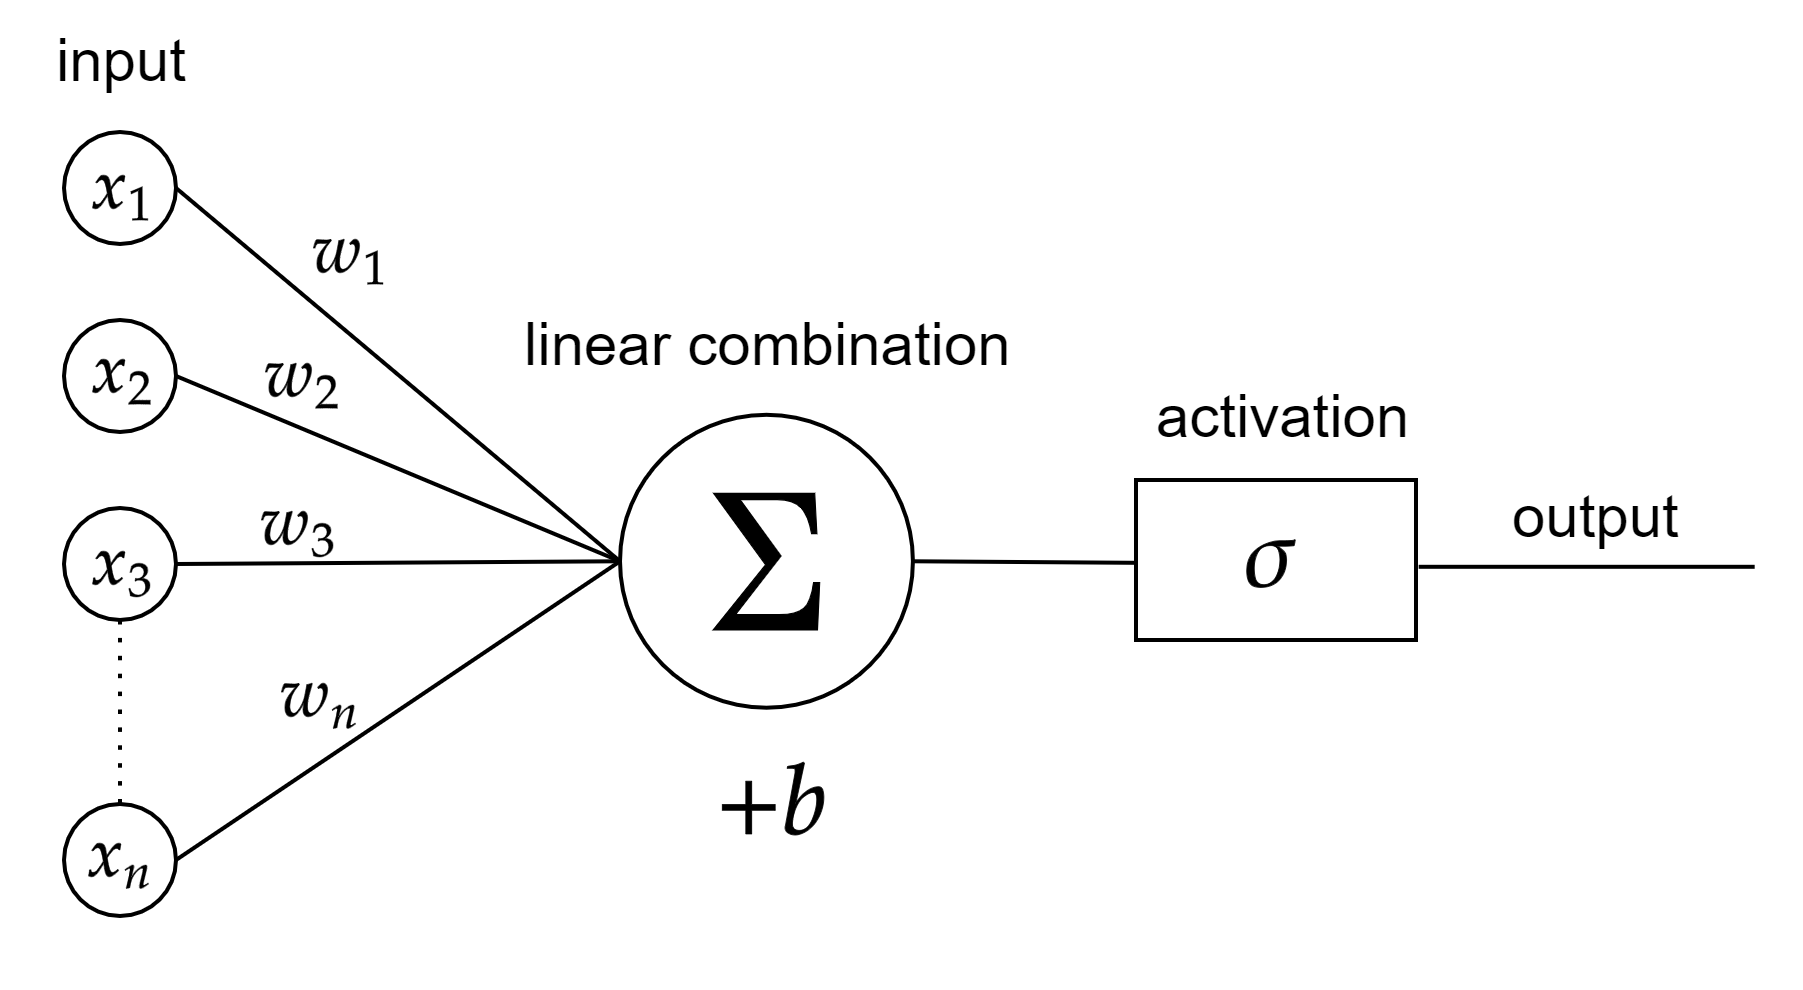
\includegraphics[scale=0.3]{img/diagram-20220205_1.png}
    \end{center}
    \caption{Illustration of the perceptron model for a single neuron.}
    \label{fig4}
\end{figure}

The choice of activation function is determined by the nature of the input and the assumed distribution of the output. When the activation function is for example equal to the Heaviside step function, i.e.
\begin{equation*}
    \sigma(x) = \begin{cases} 1 & \text{if } x \geq 0, \\ 0 & \text{if } x < 0, \end{cases}
\end{equation*}
then the perceptron coincides with a linear support vector classifier, see \cite[Chapter~7]{Bishop:2006}. \\
The activation function can be any non-constant, non-linear function, but those generally used are monotone increasing, continuous, and at least piecewise smooth. At present, the most popular activation function is the rectified linear unit, abbreviated ReLu, \cref{ReLu}. In recent decades, smoother activation functions have been used, such as the sigmoid function, \cref{Sigmoid}, or the hyperbolic tangent function, \cref{TanH}, \cite{}.
\begin{align}
    \sigma(y) &=\max \{y, 0\} & & \text{ rectified linear unit (ReLU) } \label{ReLu} \\
    \sigma(y) &=\frac{1}{1+\exp (-y)} & & \text{ sigmoid } \label{Sigmoid} \\
    \sigma(y) &=\tanh (y)=\frac{\exp (y)-\exp (-y)}{\exp (y)+\exp (-y)} & & \text{ hyperbolic tangent } \label{TanH}
\end{align}
A single perceptron can already be understood as a neural network, but it still has many limitations. Above all, the dimension of the output is limited to $1$. If one wants to create a multi-dimensional output, one arranges several perceptrons in a layer by distributing the input to exactly as many perceptrons as one needs the dimension of the output. Suppose the input has dimension $n$ and the output should have dimension $m$. The weights of the $m$ neurons on that layer can be conveniently organized into a matrix a matrix $W \in \mathbb{R}^{m \times n}$, where each row corresponds to the $n$ weights of each perceptron, i.e. $w^{i} \in \mathbb{R}^n$ for all $i = 1, \ldots, m$. The biases of the $m$ perceptrons are represented as a vector $b \in \mathbb{R}^m$. The weighted sum of the input $x \in \mathbb{R}^n$ with the addition of a bias for each perceptron can be computed as  
\begin{equation*}
    a = W x + b \in \mathbb{R}^m,
\end{equation*}
which is often referred as propagation function. To simplify the notation, we define the activation function $\sigma \colon \mathbb{R} \to \mathbb{R}$ for vector-valued input values $a \in \mathbb{R}^m$ by applying it component-wise: 
\begin{equation*}
    \sigma \colon \mathbb{R}^{m} \ni a \mapsto \sigma(a):= \left(
        \begin{array}
            {c} \sigma \left( a_{1} \right) \\
            \vdots \\
            \sigma\left(a_{m}\right)
        \end{array}
        \right) \in \mathbb{R}^{m}.
\end{equation*}
Unfortunately, the ability of a single layer of perceptrons to model any reasonably complicated function is not very pronounced. This led to the idea of connecting several such layers of neurons one after the other, and utilizing the outputs from one layer of neurons as inputs to the neurons of the subsequent layer. From now on, we will refer to such a composition of layers of artificial neurons as a neural network. \\
We assume that we have $L \in \mathbb{N}$ layers of artificial neurons and we would like to connect them one after the other. Let us consider one layer of artificial neurons. We use n to denote the number of neurons in layer l. We denote the weight matrix by W and the bias by b. The matrix has n columns and m rows because it receives the output from the l-1 layer as input for the l layer and must generate nl linear combinations for the neurons in the l layer. The activation function can also depend on the layer, which is why we denote it with sigma. To simplify the notation, we introduce another layer to identify the input, which we will call the input layer. The number of neurons in this layer corresponds to the dimension of the input. This layer does not change the input and is the first layer of the network. The last layer of a neural network is called the output layer, whose number of neurons is equal to the desired dimension of the output. All other layers are called hidden layers. \\
A neural network now processes information as follows: The input from the input layer is passed to the first layer. 

The first layer has n neurons. Like the single layer shown above, it first calculates a matrix vector product with W and the input, adds a bias to it and applies an activation function to the activation in this first layer, so that the layer l=1 returns a vector z. This vector z is passed to layer 2 and the whole process is repeated until the last layer is reached.  


\begin{figure}[H]
    \begin{center}
        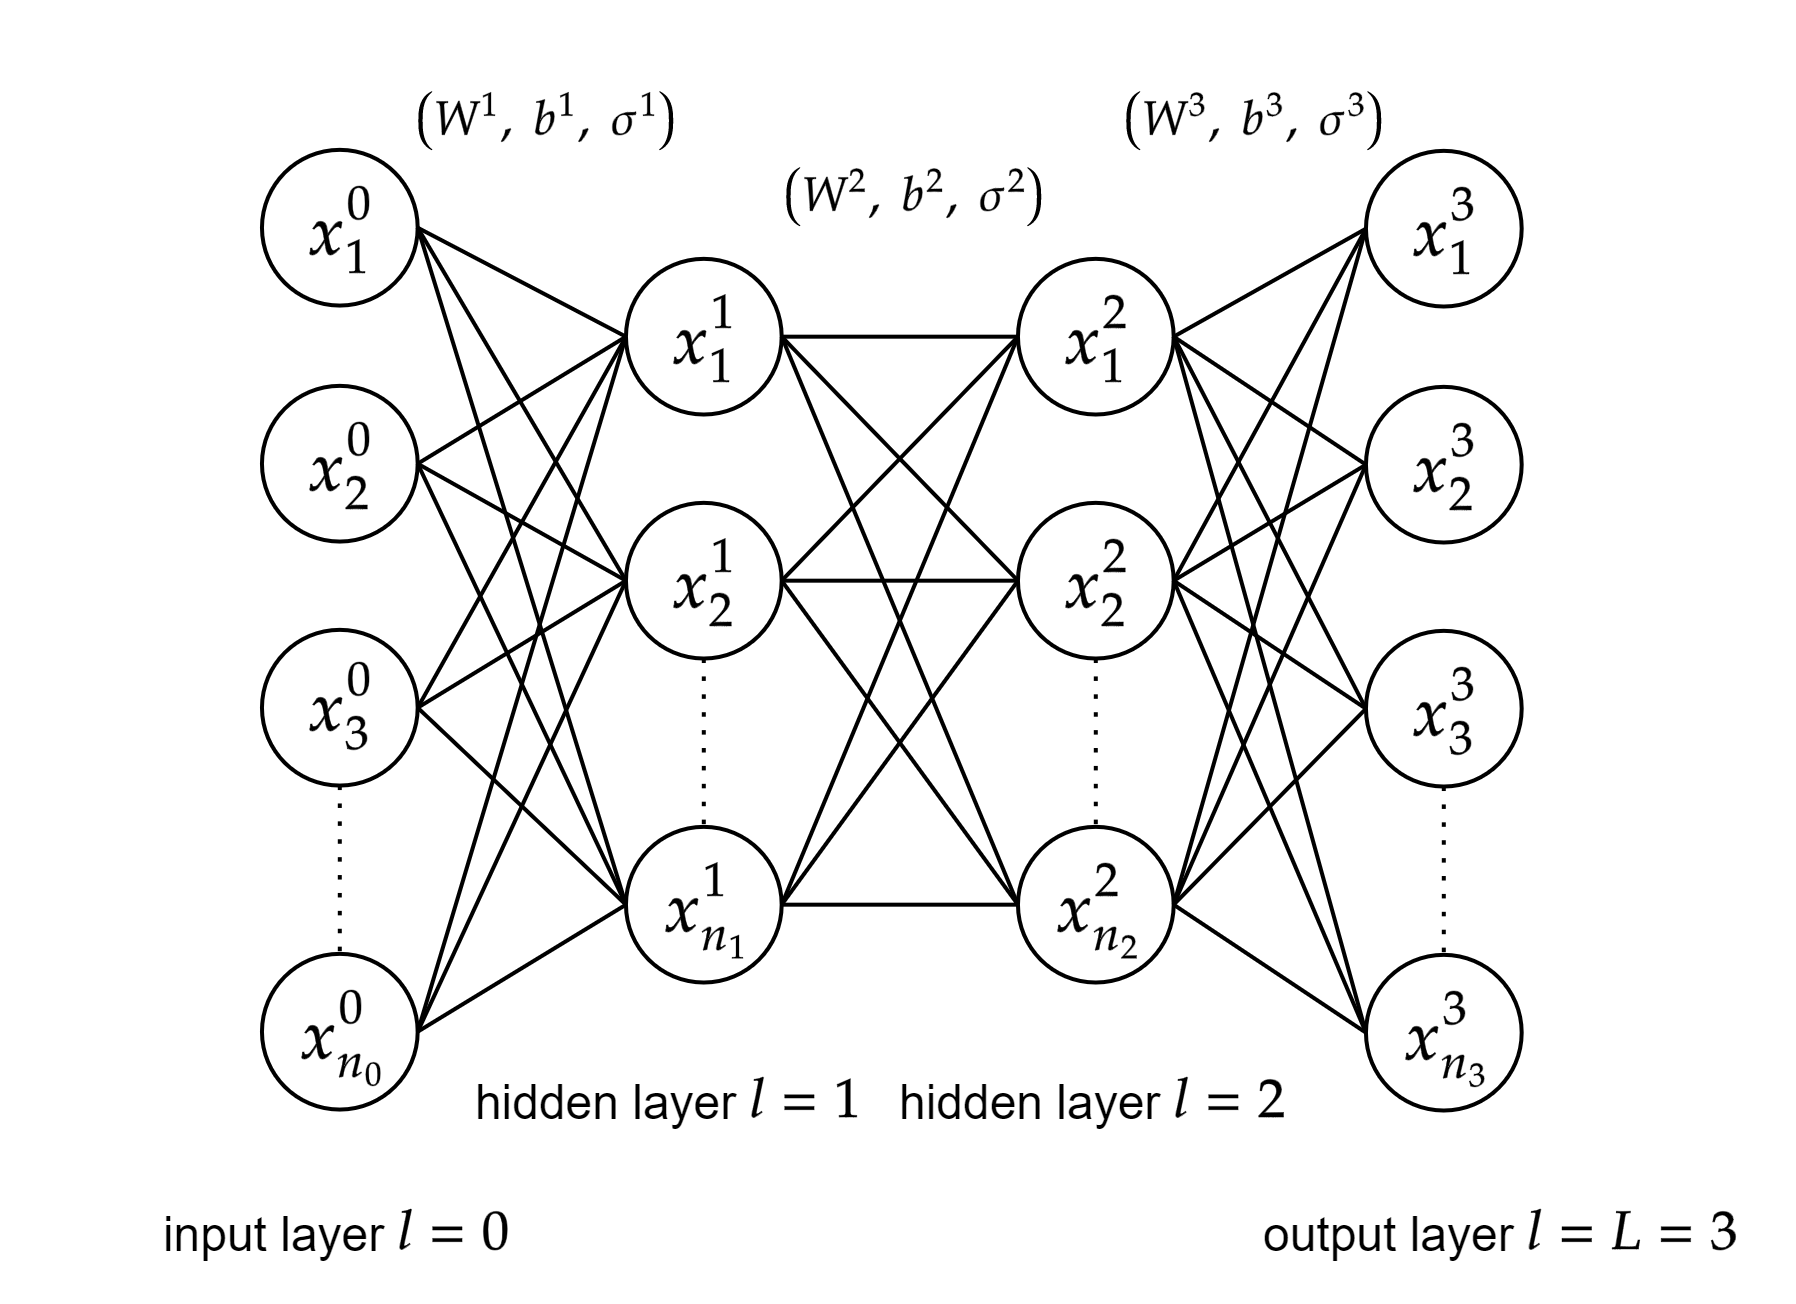
\includegraphics[scale=0.3]{img/diagram-20220206.png}
    \end{center}
    \caption{Illustration of an artificial neural network with $L=3$ layers.}
    \label{fig5}
\end{figure}

\begin{equation*}
    \mathbb{R}^{n^{(\ell-1)}} \ni \underbrace{x^{(\ell-1)}}_{\text {input of layer } \ell} \mapsto x^{(\ell)}:=\underbrace{\sigma^{(\ell)}\left(\left(W^{(\ell)}\right)^{\top} x^{(\ell-1)}+b^{(\ell)}\right)}_{\text {output of layer } \ell}=: F^{(\ell)}\left(x^{(\ell-1)}, W^{(\ell)}, b^{(\ell)}\right) \in \mathbb{R}^{n^{(\ell)}} .
\end{equation*}


\begin{equation*}
    \begin{aligned}
        y &=\sigma^{(3)}\left(\left(W^{(3)}\right)^{\top} \sigma^{(2)}\left(\left(W^{(2)}\right)^{\top} \sigma^{(1)}\left(\left(W^{(1)}\right)^{\top} x^{(0)}+b^{(1)}\right)+b^{(2)}\right)+b^{(3)}\right) \\
        &=F^{(3)}\left(F^{(2)}\left(F^{(1)}\left(x^{(0)}, W^{(1)}, b^{(1)}\right), W^{(2)}, b^{(2)}\right), W^{(3)}, b^{(3)}\right) \\
        &=: F\left(x^{(0)}, W^{(1)}, b^{(1)}, W^{(2)}, b^{(2)}, W^{(3)}, b^{(3)}\right) .
    \end{aligned}
\end{equation*}

They are obtained by organizing perceptrons in layers ` = 1, . . . , L and utilizing the outputs from one layer of neurons as inputs to the neurons of the subsequent layer,


the feed-forward neural network, also known as the multilayer perceptron,

The process of evaluating (5.7) can then be interpreted as a forward
propagation of information through the network.

In artificial neural networks, topology refers to the structure of the network. This generally means how many artificial neurons are located on how many layers and how they are connected to each other. Artificial neurons can be connected in many ways to form an artificial neural network. In many models, neurons are arranged in layers one behind the other; 




Indeed,
it has been used very broadly to cover a wide range of different models, many of
which have been the subject of exaggerated claims regarding their biological plausibility. From the perspective of practical applications of pattern recognition, however, biological realism would impose entirely unnecessary constraints. Our focus in
this chapter is therefore on neural networks as efficient models for statistical pattern
recognition. In particular, we shall restrict our attention to the specific class of neural networks that have proven to be of greatest practical value, namely the multilayer
perceptron

Deep-learning methods are representation-learning methods with multiple levels of representation, obtained by composing simple but non-linear modules that each transform the representation at one level (starting with the raw input) into a representation at a higher, slightly more abstract level. With the composition of enough such transformations, very complex functions can be learned.

The most common form of machine learning, deep or not, is supervised learning.

The equations used for computing the forward pass in a neural net



The more complex the problem to be solved with the help of the neural network is, the more layers are needed. 

We compute an objective function that measures the error (or distance) between the output scores and the desired pattern of scores. The machine then modifies its internal adjustable parameters to reduce  this error. These adjustable parameters, often called weights, are real numbers that can be seen as ‘knobs’ that define the input–output function of the machine. In a typical deep-learning system, there may be hundreds of millions of these adjustable weights, and hundreds of millions of labelled examples with which to train the machine. To properly adjust the weight vector, the learning algorithm computes a gradient vector that, for each weight, indicates by what amount the error would increase or decrease if the weight were increased by a tiny amount. The weight vector is then adjusted in the opposite direction to the gradient vector. 

A deep-learning architecture is a multilayer stack of simple modules, all (or most) of which are subject to learning, and many of which compute non-linear input–output mappings. Each module in the stack transforms its input to increase both the selectivity and the invariance of the representation.

The backpropagation procedure to compute the gradient of an objective function with respect to the weights of a multilayer stack of modules is nothing more than a practical application of the chain rule for derivatives. The key insight is that the derivative (or gradient) of the objective with respect to the input of a module can be computed by working backwards from the gradient with respect to the output of that module

Many applications of deep learning use feedforward neural network architectures (Fig. 1), which learn to map a fixed-size input (for example, an image) to a fixed-size output (for example, a probability for each of several categories). To go from one layer to the next, a set of units compute a weighted sum of their inputs from the previous layer and pass the result through a non-linear function. At present, the most popular non-linear function is the rectified linear unit (ReLU), which is simply the half-wave rectifier. In past decades, neural nets used smoother non-linearities, such as , but the ReLU typically learns much faster in networks with many layers, allowing training of a deep supervised network without unsupervised pre-training28. Units that are not in the input or output layer are conventionally called hidden units. The hidden layers can be seen as distorting the input in a non-linear way so that categories become linearly separable by the last layer 



Perceptron
Activation Function
One layer
Neural Network
FNN
%ResNet
Machine Learning, Training 
Supervised Learning
Unsupervised Learning
Gradient Based optimization
Backpropagation 
Honrik 